\documentclass[tikz,border=5pt]{standalone}
\usepackage{luatexja}
\usepackage[hiragino-pron]{luatexja-preset}
\usepackage{amsmath,amssymb}
\usetikzlibrary{arrows.meta,patterns}

\begin{document}
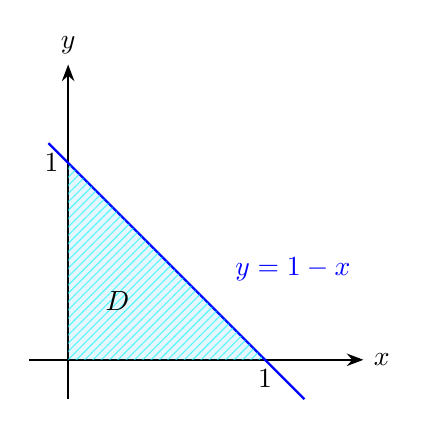
\begin{tikzpicture}[scale=2.5]

% Axes
\draw[-{Stealth[length=6pt]}, thick] (-0.2,0) -- (1.5,0) node[right] {$x$};
\draw[-{Stealth[length=6pt]}, thick] (0,-0.2) -- (0,1.5) node[above] {$y$};

% Line y = 1 - x
\draw[thick, blue, domain=-0.1:1.2, samples=2] plot (\x, {1-\x});

% Fill region D (triangle)
\fill[pattern=north east lines, pattern color=cyan, opacity=0.6]
  (0,0) -- (1,0) -- (0,1) -- cycle;
\fill[cyan, opacity=0.1]
  (0,0) -- (1,0) -- (0,1) -- cycle;

% Labels
\node[below] at (1,0) {$1$};
\node[left] at (0,1) {$1$};
\node at (0.25,0.3) {$D$};
\node[above right, blue] at (0.8,0.35) {$y = 1 - x$};

\end{tikzpicture}
\end{document}
